\documentclass[12pt, titlepage]{article}

\usepackage{amsmath, mathtools}
\usepackage{amsfonts}
\usepackage{amssymb}
\usepackage{graphicx}
\usepackage{colortbl}
\usepackage{xr}
\usepackage{hyperref}
\usepackage{longtable}
\usepackage{xfrac}
\usepackage{tabularx}
\usepackage{siunitx}
\usepackage{booktabs}
\usepackage{caption}
\usepackage{multirow}
\usepackage{pdflscape}
\usepackage{afterpage}
\usepackage[table,xcdraw]{xcolor}
\hypersetup{
    colorlinks,
    citecolor=blue,
    filecolor=black,
    linkcolor=red,
    urlcolor=blue
}
\usepackage[round]{natbib}

%% Comments

\usepackage{color}

\newif\ifcomments\commentstrue %displays comments
%\newif\ifcomments\commentsfalse %so that comments do not display

\ifcomments
\newcommand{\authornote}[3]{\textcolor{#1}{[#3 ---#2]}}
\newcommand{\todo}[1]{\textcolor{red}{[TODO: #1]}}
\else
\newcommand{\authornote}[3]{}
\newcommand{\todo}[1]{}
\fi

\newcommand{\wss}[1]{\authornote{blue}{SS}{#1}} 
\newcommand{\plt}[1]{\authornote{magenta}{TPLT}{#1}} %For explanation of the template
\newcommand{\an}[1]{\authornote{cyan}{Author}{#1}}

%% Common Parts

\newcommand{\progname}{Optimal EM Placement} % PUT YOUR PROGRAM NAME HERE
\newcommand{\authname}{Hussein Saad} % AUTHOR NAMES                  

\usepackage{hyperref}
    \hypersetup{colorlinks=true, linkcolor=blue, citecolor=blue, filecolor=blue,
                urlcolor=blue, unicode=false}
    \urlstyle{same}
                                


% For easy change of table widths
\newcommand{\colZwidth}{1.0\textwidth}
\newcommand{\colAwidth}{0.13\textwidth}
\newcommand{\colBwidth}{0.82\textwidth}
\newcommand{\colCwidth}{0.1\textwidth}
\newcommand{\colDwidth}{0.05\textwidth}
\newcommand{\colEwidth}{0.8\textwidth}
\newcommand{\colFwidth}{0.17\textwidth}
\newcommand{\colGwidth}{0.5\textwidth}
\newcommand{\colHwidth}{0.28\textwidth}

\begin{document}

\title{System Verification and Validation Plan for \progname{}} 
\author{\authname}
\date{\today}
	
\maketitle

\pagenumbering{roman}

\section*{Revision History}

\begin{tabularx}{\textwidth}{p{3.5cm}p{2cm}X}
\toprule {\bf Date} & {\bf Version} & {\bf Notes}\\
\midrule
April 16, 2025 & 1.3 & Change output test cases\\
\midrule
April 15, 2025 & 1.2 & Implement  instructor suggestions\\
\midrule
April 13, 2025 & 1.1 & Implement domain expert suggestions\\
\midrule
February 23, 2025 & 1.0 & Initial draft\\
\bottomrule
\end{tabularx}


\newpage

\tableofcontents
\newpage

\section{Symbols, Abbreviations, and Acronyms}

\renewcommand{\arraystretch}{1.2}
\begin{tabular}{l l} 
  \toprule		
  \textbf{symbol} & \textbf{description}\\
  \midrule 
  T & Test\\
  EM & Electromagnet\\
  VnV & Verification and Validation \\
  SRS & Software Requirements Specification \\
  PV & Positive value required \\
  TL & Input parameter too large \\
  IT & Invalid type \\
  \bottomrule
  \label{abbrevs}
\end{tabular}\\

\newpage

\pagenumbering{arabic}

This document provides the road-map of the verification and validation plan for Optimal EM Placement. The plan ensures the requirements and models in the SRS document are correctly implemented. It starts with introducing general information about the program in Section \ref{gen_info}, followed by a plan, and then an outline of system tests in Section \ref{sys_tests}. Finally, a description of unit tests for functional and non-functional requirements is provided in Section \ref{unit_tests}.

\section{General Information} \label{gen_info}

\subsection{Summary}
This document outlines the verification and validation plan for Optimal EM Placement, a program that calculates the optimal positions of EM actuators that yield the highest system manipulability, as defined in the \href{https://github.com/husseinsd1/optimal-em-arrangement/blob/main/docs/SRS/SRS.pdf}{SRS}. 

\subsection{Objectives}
The main purpose of this document is to define how validation will be performed for the requirements outlined in the \href{https://github.com/husseinsd1/optimal-em-arrangement/blob/main/docs/SRS/SRS.pdf}{SRS} document. The verification plan includes strategies to ensure the correct execution of system requirements testing. In particular, the VnV document devises procedures to confirm that intermediate data and computations are approximately correct, and conform to the theoretical expectations laid out in the SRS. The optimal EM positions are solved for by the \href{https://www.cvxpy.org/}{$\texttt{cvxpy}$} library --- a popular open-source convex optimization library --- which is assumed to be reliable and correct for the purposes of this project. In general, we aim to build maximum confidence in the correctness of our program. Additionally, the document outlines methods to verify that the input interface and output format are sufficiently accessible and interpretable by the intended users, as defined in the SRS. However, extensive usability verifications, beyond what is necessary for the outlined user backgrounds, is not within scope of this project.

\subsection{Challenge Level and Extras}
This project is an advanced project as it is the product of research work that will later be submitted for publication in an academic conference/journal.  

\subsection{Relevant Documentation}
The \href{https://github.com/husseinsd1/optimal-em-arrangement/blob/main/docs/ProblemStatementAndGoals/ProblemStatement.pdf}{Problem Statement} motivates the program while the \href{https://github.com/husseinsd1/optimal-em-arrangement/blob/main/docs/SRS/SRS.pdf}{SRS} provides information about the requirements of the functioning program. The \href{https://github.com/husseinsd1/optimal-em-arrangement/blob/main/docs/Design/SoftArchitecture/MG.pdf}{MG} and \href{https://github.com/husseinsd1/optimal-em-arrangement/blob/main/docs/Design/SoftDetailedDes/MIS.pdf}{MIS} documents contain architecture and design rationale. 

\section{Plan}
This section outlines the testing plan for the Optimal EM Placement program, starting with the team in Section \ref{team}, followed by the SRS verification plan, design verification plan, VnV verification plan, implementation verification plan, automated testing, ending with verification tools in Section~\ref{ver_tools}.

\subsection{Verification and Validation Team} \label{team}
% \begin{table}[]
%   \begin{tabular}{|c|c|c|c|}
%     \hline
%     \rowcolor[HTML]{FFC702} 
%     Name & Document & Role               & Description                                         \\ \hline
%     Hussein Saad & All      & Author             & Execution and management of VnV document and tests. \\ \hline
%     Dr. Spencer Smith & All      & Instructor         & Review all documents.                               \\ \hline
%     Uriel Cruz & All      & Domain Expert      & Review document and provide technical feedback.     \\ \hline
%     Alaap Grandhi & VnV      & Secondary Reviewer & Review the VnV plan and suggest improvements.       \\ \hline
%   \end{tabular}
% \end{table}
\begin{center}
  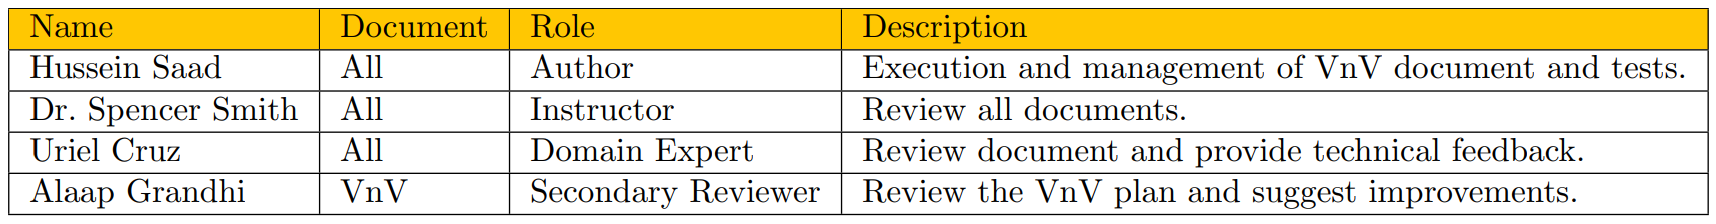
\includegraphics[scale=0.36]{VnVTeam.PNG} \label{team_table}
  \captionof{table}{Verification Team}
\end{center}

\subsection{SRS Verification Plan}
The Optimal EM Placement SRS document will be verified primarily through ad hoc feedback from reviewers. Document design and alignment with course goals will be reviewed by the instructor (Dr.~Spencer Smith), while more technical details will benefit from the comments of the Domain Expert Reviewer (Uriel Cruz) and the External Reviewer (Dr.~Matthew Giamou). After the creation/update of the SRS document, reviewers will provide the author with feedback through GitHub issues. The author will implement the suggested changes as necessary. In addition, the \href{https://github.com/husseinsd1/optimal-em-arrangement/blob/main/docs/Checklists/SRS-Checklist.pdf}{SRS checklist} created by Dr.~Smith will be used to be used to verify that the document adheres to all specified criteria. Consequently, both reviewer feedback and the checklist will ensure that the SRS meets the necessary technical and design standards.

\subsection{Design Verification Plan}
The design documents, Module Guide (MG) and Module Interface Specification (MIS), will be verified through inspection by reviewers. The \href{https://github.com/husseinsd1/optimal-em-arrangement/blob/main/docs/Checklists/MG-Checklist.pdf}{MG checklist} and \href{https://github.com/husseinsd1/optimal-em-arrangement/blob/main/docs/Checklists/MIS-Checklist.pdf}{MIS checklist} by Dr.~Smith will serve as a reference for reviewers. 

\subsection{Verification and Validation Plan Verification Plan}
The Verification and Validation Plan will itself be verified primarily through manual reviews by the Instructor, Domain Expert, and Secondary Reviewer. Reviewers will compare the document against the criteria specified by Dr~.Smith in the \href{https://github.com/husseinsd1/optimal-em-arrangement/blob/main/docs/Checklists/VnV-Checklist.pdf}{VnV checklist}.

\subsection{Implementation Verification Plan}
The implementation of Optimal EM Placement will be verified primarily in two different ways:
\begin{enumerate}
  \item \textbf{Code Walkthrough (Static): }Walkthroughs will be performed by the author, domain expert, and secondary reviewer. The reviewers will run and interact with the program, checking for bugs and vulnerabilities in the code. Static analysis tools like \href{https://github.com/pylint-dev/pylint}{\texttt{Pylint}} can be used to examine the code for smells and potential refactoring opportunities. This process is followed by a discussion in which members discuss their findings and suggest enhancements.  
  \item \textbf{Test Cases (Dynamic): }As outlined in Section \ref{sys_tests}, test cases will be executed to verify the function and non-functional requirements mentioned in the SRS. 
\end{enumerate}

\subsection{Automated Testing and Verification Tools} \label{ver_tools}
Automated testing as outlined in the previous section will be carried out using the \href{https://docs.pytest.org/en/stable/}{\texttt{PyTest}} library, by comparing expected outputs to calculated outputs given some constant user input. 

\section{System Tests} \label{sys_tests}

\subsection{Tests for Functional Requirements}
The functional and nonfunctional requirements of the program are given in Sections 5.1 and 5.2 of the \href{https://github.com/husseinsd1/optimal-em-arrangement/blob/main/docs/SRS/SRS.pdf}{SRS}. The relationship between test cases and requirements is given in the traceability matrix in Section \ref{trac_matrix}. \\ \\
\noindent \emph{Error codes in Table \ref{emprop} are explained in Section \ref{abbrevs} of the document.}


\subsubsection{Input Tests - Invalid Input}

		
\paragraph{Incorrect EM Properties}
\begin{center}
  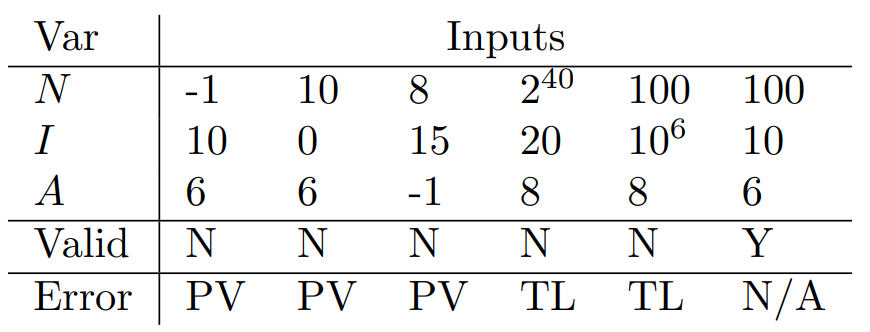
\includegraphics[scale=0.6]{EMInputTable.PNG} \\
  \captionof{table}{EM properties test cases}
  \label{emprop}
\end{center}

\begin{enumerate}

\item{test-em-props-1\dots6\\}

Control: Automatic.
					
Initial State: Pending input.
					
Input: Set of input values for EM Properties as given in Table \ref{emprop}.
					
Output: An appropriate error message, if necessary, as given in Table \ref{emprop}.

Test Case Derivation: These cases test the behaviour of the system when given invalid system related inputs as described in Table 2 of the SRS.
					
How test will be performed: Using \texttt{PyTest}. 
\end{enumerate}

\newpage

\paragraph{Invalid Input Type}
\begin{center}
  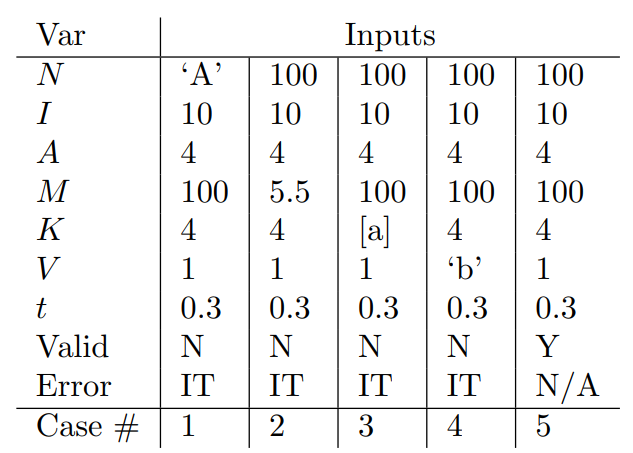
\includegraphics[scale=0.5]{InvTypeTable.PNG} \\
  \captionof{table}{Input type test cases}
  \label{inp_type_table}
\end{center}

\begin{enumerate}

  \item{test-inp-type-1\dots5\\}
  
  Control: Automatic.
            
  Initial State: Pending input.
            
  Input: Set of input values for the system as given in Table \ref{inp_type_table}.
            
  Output: An appropriate error message, if necessary, as given in Table~\ref{inp_type_table}.
  
  Test Case Derivation: These cases test the behaviour of the system when given invalid input types, based on what is described in the SRS.
            
  How test will be performed: Using \texttt{PyTest}. 
\end{enumerate}

\newpage

\paragraph{System Setup}
\begin{center}
  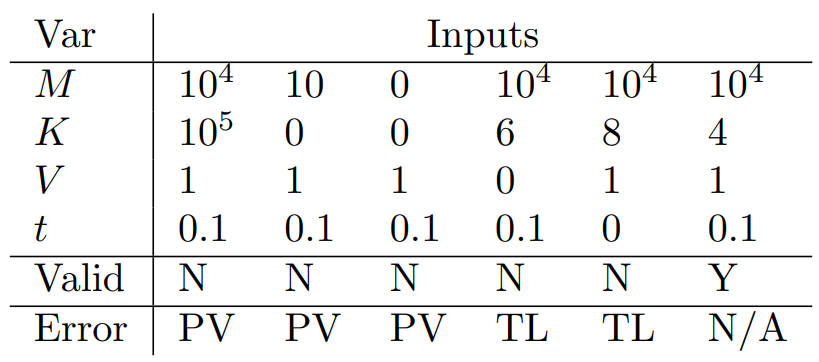
\includegraphics[scale=0.49]{SysInputTable.PNG} \\
  \captionof{table}{System setup test cases}
  \label{sys_setup_table}
\end{center}

\begin{enumerate}

  \item{test-sys-setup-1\dots6\\}
  
  Control: Automatic.
            
  Initial State: Pending input.
            
  Input: Set of input values for the system as given in Table \ref{sys_setup_table}.
            
  Output: An appropriate error message, if necessary, as given in Table~\ref{sys_setup_table}.
  
  Test Case Derivation: These cases test the behaviour of the system when given invalid EM related inputs as described in Table 2 of the SRS.
            
  How test will be performed: Using \texttt{PyTest}. 
\end{enumerate}

\newpage

\subsubsection{Output Tests - Correct Output}
\paragraph{Correct Positions Selected}
\begin{center}
  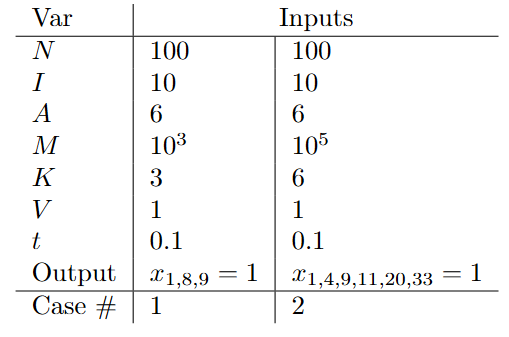
\includegraphics[scale=0.4]{OutputTable.PNG} \\
  \captionof{table}{Output correctness test cases}
  \label{output_tests_table}
\end{center}

\begin{enumerate}

  \item{test-output-correct-1\dots2\\}
  
  Control: Automatic.
            
  Initial State: Pending input.
            
  Input: Set of input values for as given in Table~\ref{output_tests_table}.
            
  Output: A binary vector $x$, such that the values at the indices shown in Table~\ref{output_tests_table} are 1. An value equalling 1 at an index, indicates an EM actuator taking the pose at that index.

  Note: The above must hold for a set of randomly generated poses with a \texttt{numpy} \texttt{default\_rng} of 123. 
  
  Test Case Derivation: These cases ensure the system returns the correct optimal positions based on the inputs it receives. 
            
  How test will be performed: Using \texttt{PyTest}. 
\end{enumerate}

\subsubsection{Intermediate Tests - Intermediate Computations} \label{svd_test}
\paragraph{Singular Values}

\begin{enumerate}

  \item{test-intmed-svd-1\dots2\\} 
  
  Control: Automatic.
            
  Initial State: Pending input.
            
  Input: Set of input values as given in Table \ref{output_tests_table}.
            
  Output: Approximately $11242$, $32600$ for test-intmed-svd-1 and test-intmed-svd-2 respectively. These values correspond to the lowest singular value of the $\mathcal{U}$ matrix described in Section 4.2.4 of the SRS.
  
  Test Case Derivation: These cases ensure the program is correctly constructing the $\mathcal{U}$ matrix and computing the magnetic field and force values. 
            
  How test will be performed: Using \texttt{PyTest}. 
\end{enumerate}

\subsection{Tests for Nonfunctional Requirements} \label{test_nfr}
The 4 nonfunctional requirements for Optimal EM placement is given in Section 5.2 of the SRS. 
\subsubsection{Accuracy}
\begin{enumerate}

\item{test-nf-acc\\}

Type: Manual.
					
Initial State: Pending input.
					
Input: Various.
					
Output: An array of lowest singular values from 100 runs.
					
How test will be performed: The author will use various parameters on the OEMP, greedy and random algorithms, and plot a singular value distribution from the 100 runs to compare performance, as explained in NF1 of the SRS. This test related to the Singular Values test in \ref{svd_test}. The average minimum singular value across OEMP runs must be at least 50\% greater than that of greedy runs. 
\end{enumerate}

\subsubsection{Usability}
\begin{enumerate}

\item{test-nf-use\\}

Type: Manual.
					
Initial State: None.
					
Input: None.
					
Output: None.
					
How test will be performed: A group of users will be asked to use the system and attempt to get a solution for their inputs. They will then answer the questions provided in the \hyperref[use_survey]{Usability Survey}. An average score of 7 or above indicates the user found the program satisfactorily usable.

\end{enumerate}

\subsubsection{Maintainability}
\begin{enumerate}

\item{test-nf-mtn\\}

Type: Static.
					
Initial State: None.
					
Input: None.
					
Output: None.
					
How test will be performed: The author will meet with the Domain Expert Reviewer and Secondary Reviewer to present a code walkthrough and discuss details related to software maintainability, in particular: the modularity of the code, the comprehensiveness of the test cases, and the consistency of formatting. 
\end{enumerate}

\subsubsection{Portability}
\begin{enumerate}

\item{test-nf-prt\\}

Type: Manual.
					
Initial State: None.
					
Input: None.
					
Output: None.
					
How test will be performed: The author will manually run all tests listed in this document on a Windows, MacOS and Linux machine. 
\end{enumerate}

\subsection{Traceability Between Test Cases and Requirements} \label{trac_matrix}
Traceability between tests and requirements is visualized below:
\begin{center}
  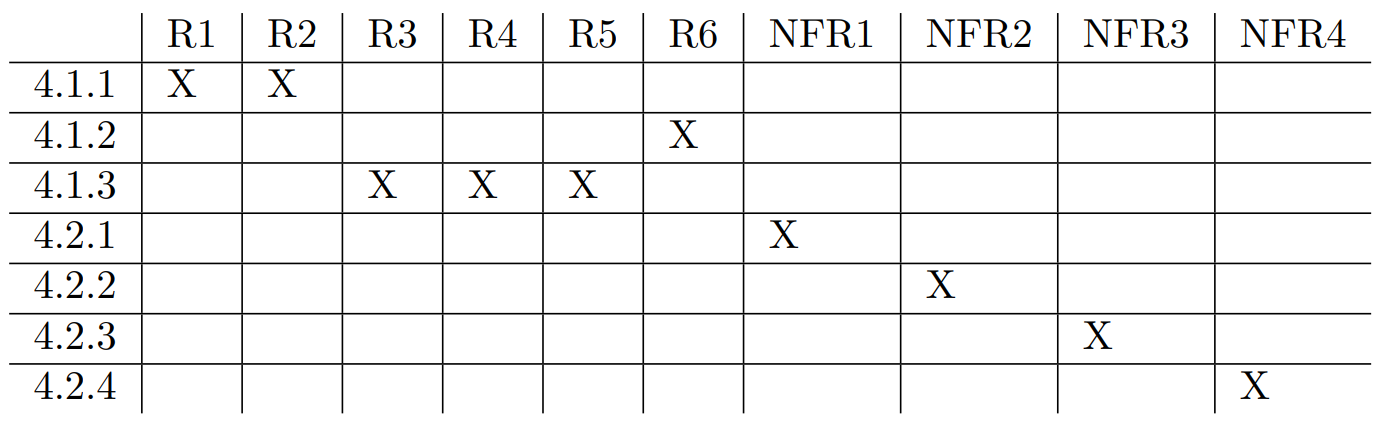
\includegraphics[scale=0.4]{TraceabilityMatrix.PNG}
  \captionof{table}{Traceability between tests and requirements}
\end{center}




%%%%%%%%%%%%%%%%%%%%%%%%%%%%%%%%%%%%%%%%%%%%






\newpage
\section{Unit Test Description} \label{unit_tests}
OEMP source code contains the following modules:
\begin{itemize}
  \item ConstantParams.py - corresponds to Section 6 of the \href{https://github.com/husseinsd1/optimal-em-arrangement/blob/main/docs/Design/SoftDetailedDes/MIS.pdf}{MIS}.
  \item InputParameters.py corresponds to Section 7 of the \href{https://github.com/husseinsd1/optimal-em-arrangement/blob/main/docs/Design/SoftDetailedDes/MIS.pdf}{MIS}.
  \item MagneticMoment.py - corresponds to Section 8 of the \href{https://github.com/husseinsd1/optimal-em-arrangement/blob/main/docs/Design/SoftDetailedDes/MIS.pdf}{MIS}.
  \item MagneticField.py - corresponds to Section 9 of the \href{https://github.com/husseinsd1/optimal-em-arrangement/blob/main/docs/Design/SoftDetailedDes/MIS.pdf}{MIS}.
  \item MagneticForce.py - corresponds to Section 10 of the \href{https://github.com/husseinsd1/optimal-em-arrangement/blob/main/docs/Design/SoftDetailedDes/MIS.pdf}{MIS}.
  \item GeneratePoses.py - corresponds to Section 11 of the \href{https://github.com/husseinsd1/optimal-em-arrangement/blob/main/docs/Design/SoftDetailedDes/MIS.pdf}{MIS}.
  \item ActuationMatrix.py - corresponds to Section 12 of the \href{https://github.com/husseinsd1/optimal-em-arrangement/blob/main/docs/Design/SoftDetailedDes/MIS.pdf}{MIS}.
  \item OptimalPlacement.py - corresponds to Section 13 of the \href{https://github.com/husseinsd1/optimal-em-arrangement/blob/main/docs/Design/SoftDetailedDes/MIS.pdf}{MIS}.
  \item OutputResults.py - corresponds to Section 14 of the \href{https://github.com/husseinsd1/optimal-em-arrangement/blob/main/docs/Design/SoftDetailedDes/MIS.pdf}{MIS}.
  \item Main.py - corresponds to Section 15 of the \href{https://github.com/husseinsd1/optimal-em-arrangement/blob/main/docs/Design/SoftDetailedDes/MIS.pdf}{MIS}.
\end{itemize}

\subsection{Unit Testing Scope}
Unit testing will be performed for the following modules: 
\begin{itemize}
  \item InputParameters.py 
  \item ActuationMatrix.py
\end{itemize}
These are high priority modules that are fundamental to the correct and successful execution of the program. The correctness of the ActuationMatrix.py module corresponds to the correctness of the MagneticMoment.py, MagneticField.py and MagneticForce.py modules (see Section 12.4.4 of the \href{https://github.com/husseinsd1/optimal-em-arrangement/blob/main/docs/Design/SoftDetailedDes/MIS.pdf}{MIS}). Higher-level modules (e.g. OptimalPlacement.py) rely on complex solver behavior and will be validated at the system-test level. Other low-level modules like ConstantParams.py, GeneratePoses.py and OutputResults.py perform trivial procedures, some using external libraries (e.g. Numpy, SciPy), and need not be unit tested. 


\subsection{Tests for Functional Requirements}
Not applicable as all modules are directly or indirectly tested through system or unit tests. 

\subsection{Tests for Nonfunctional Requirements}
Not applicable. Empirically verifiable non-functional requirements are tested through system tests (see Section \ref{test_nfr}).

\subsection{Traceability Between Test Cases and Modules}
Traceability between test cases and modules is given below:



\newpage

\bibliographystyle{plainnat}

\bibliography{../../refs/References}

\newpage

\section{Appendix}

This is where you can place additional information.

\subsection{Symbolic Parameters}

The definition of the test cases will call for SYMBOLIC\_CONSTANTS.
Their values are defined in this section for easy maintenance.

\subsection{Usability Survey Questions} \label{use_survey}
Answer the following questions one a scale of 1 to 10 (where 1 is ``very poor'' and 10 is ``excellent''):
\begin{itemize}
  \item How easy was it to understand and use the program's input fields?
  \item How useful are the error messages or feedback provided when an incorrect input is given?
  \item How would you rate the overall flow between input and output interactions during your usage?
  \item How clear and helpful is the output produced by the program?
  \item How satisfied are you with the overall interaction experience of the program?
\end{itemize}

\end{document}